\documentclass{beamer}
\mode<presentation>


\usepackage[brazil]{babel}
\usepackage[utf8]{inputenc}
 


\usepackage{amsfonts}
\usepackage{amssymb}
\usepackage{amsmath}
\usepackage{algorithm}
\usepackage{algpseudocode}



\usepackage{ae}
\usepackage{graphicx,color}
\usepackage[all]{xy}
\usepackage{empheq}
\usepackage{fancybox}
\usepackage{textcomp}
\usepackage[all]{xy}
\usepackage{textpos}
\usepackage{multicol}
\usepackage{cancel}
\usepackage{listings}
\usepackage{xcolor}
\usepackage{enumerate}
\usepackage{minted}

\usepackage[style=verbose]{biblatex}
\addbibresource{bibtex.bib}

\usepackage{tikz}
\usetikzlibrary{shapes.geometric, arrows}


\tikzstyle{startstop} = [rectangle, rounded corners, minimum width=3cm, minimum 
\tikzstyle{io} = [trapezium, trapezium left angle=70, trapezium right angle=110, minimum width=3cm, minimum height=1cm, text centered, draw=black, fill=blue!30]
\tikzstyle{process} = [rectangle, minimum width=3cm, minimum height=1cm, text centered, draw=black, fill=orange!30]
\tikzstyle{decision} = [diamond, minimum width=3cm, minimum height=1cm, text centered, draw=black, fill=green!30]
\tikzstyle{arrow} = [thick,->,>=stealth]

\newcommand{\floor}[1]{$\lfloor$ #1 $\rfloor$}

\newcommand\Fontvi{\fontsize{9}{7.2}\selectfont}



\usetheme{Boadilla}

\newcommand{\PC}[1]{\ensuremath{\left(#1\right)}}


\newcommand*{\colorboxed}{}
\def\colorboxed#1#{%
  \colorboxedAux{#1}%
}
\newcommand*{\colorboxedAux}[3]{%
  % #1: optional argument for color model
  % #2: color specification
  % #3: formula
  \begingroup
    \colorlet{cb@saved}{.}%
    \color#1{#2}%
    \boxed{%
      \color{cb@saved}%
      #3%
    }%
  \endgroup
}



\title {Pensando Computacionalmente}

\author[Wladimir Araújo Tavares]{ Wladimir Araújo Tavares$^{1}$  }

\institute[UFC]{$^{1}$Universidade Federal do Ceará - Campus de Quixadá\\}
\date{}
\AtBeginSection[]
{
  \begin{frame}<beamer>{}
    \small
    \tableofcontents[currentsection,currentsubsection]
  \end{frame}
}
\begin{document}

\begin{frame}
	\titlepage
\end{frame}

%%%%%%%%%%%%%%%%%%%%%%%%%%%%%%%%%%%%%%%%%%%%%%%%%%%%%%%%%%%%%%%%%%%%



\begin{frame}{Moeda Falsa}

\begin{itemize}
\item \textbf{Objetivos:} Desenvolver o pensamento computacional.

\item \textbf{Público-alvo:}  Alunos a partir do primeiro ano do Ensino Médio.

\item \textbf{Conteúdo:} Comando condicional e fluxograma

\item \textbf{Tempo:} 50 minutos

\item \textbf{Recursos:} Papel e Caneta

\end{itemize}
    
\end{frame}




\begin{frame}{Passo 1 - Apresentação}

\begin{itemize}
   
\item <1->Nesta atividade, você recebe um conjunto de 8 cartões circulares numerados representando moedas. No outro lado dos cartões, escreveremos um número representando o peso da moeda. No nosso problema, escreveremos o número 1 em 7 cartões e o número 2 no cartão restante.




\begin{center}
\begin{tikzpicture}
\node[circle, draw] (problema) at (0,0){1};
\node[circle, draw] (candidato) at (1,0) {2};
\node[circle, draw] (teste) at (2,0) {3};
\node[circle, draw] (teste) at (3,0) {4};
\node[circle, draw] (teste) at (4,0) {5};
\node[circle, draw] (teste) at (5,0) {6};
\node[circle, draw] (teste) at (6,0) {7};
\node[circle, draw] (teste) at (7,0) {8};

\end{tikzpicture}
\end{center}


\item <2->A tarefa é encontrar a moeda falsa (mais pesada) usando uma balança de prato realizando o mínimo de pesagens



\end{itemize}

\end{frame}


\begin{frame}{Passo 1 - Apresentação da atividade}


\begin{itemize}
    \item Uma pesagem consiste em colocar uma quantidade de moedas de um lado e a mesma quantidade de moedas do outro lado. O resultado da pesagem pode ser de três tipos:
    \begin{itemize}
        \item lado esquerdo mais pesado.
        \item lado direito mais pesado.
        \item equilibrado
    \end{itemize}
    
    
    
\begin{figure}
\begin{center}
	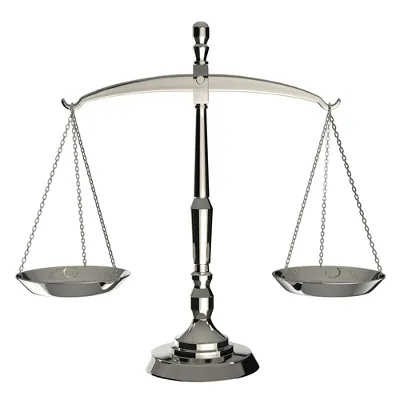
\includegraphics[scale=0.3]{images/balanca.png} 
\end{center}
\end{figure}

 
    

\end{itemize}


\end{frame}


% The task is to select those and only those cards that need to be turned over, to
% determine whether the following conditional holds:
% If there is a d on one side,
% then there is a 3 on the other side.

% são quatro pessoas. Podemos ver o que dois deles estão bebendo, mas não quantos anos eles
% está; e podemos ver a idade de dois deles, mas não o que eles estão bebendo: 


% Bob, drinking beer.
% Mary, a senior citizen, obviously over eighteen years old.28
% Computational Logic and Human Thinking
% John, drinking cola.
% Susan, a primary school child, obviously under eighteen years old.
% In contrast with the card version of the selection task, most people solve th


\begin{frame}{Passo 1 - Apresentação da atividade}

\begin{itemize}
    \item Na nossa atividade, o aluno pode usar a seguinte instrução:
    
    \begin{itemize}
        \item Compare A , B.
        \item Compare \{1\} , \{2\}.
        \item Compare \{1,2\} , \{3,4\}.
    \end{itemize}
    
    \item O resultado da comparação será esquerda, equilibrado e direita.
\end{itemize}

\end{frame}

\begin{frame}{Passo 1 - Apresentação da atividade}

\begin{itemize}
    \item No exemplo de 8 moedas, podemos fazer a primeira pesagem da seguinte maneira:
    
    \begin{itemize}
        \item Compare \{1\} e \{2\} (sobrando 6 moedas).
        \item Compare \{1,2\} e \{3,4\} (sobrando 4 moedas).
        \item Compare \{1,2,3\} e \{4,5,6\} (sobrando 2 moedas).
        \item Compare \{1,2,3,4\} e \{5,6,7,8\} (sobrando 0 moedas).
    \end{itemize}
\end{itemize}

\end{frame}


\begin{frame}{Passo 1 - Resolvendo o problema com 2 moedas}


\end{frame}


\begin{frame}{Passo 1 - Resolvendo o problema com 3 moedas}


\end{frame}


\begin{frame}{Passo 2 - Execução da atividade}

\begin{itemize}

\item <1-> O professor pode separar a sala em duas grandes equipes.

\item <2-> Cada aluno deve fazer seu próprio fluxograma avaliando todas as possibilidades de pesagens  

\item <3-> Em seguida, cada equipe deve eleger o fluxograma que eles acreditam ser o mais correto.

\item <4-> As duas equipes podem batalhar entre si. 



\end{itemize}


\end{frame}







\begin{frame}{Passo 3 - Discussão e Avaliação}

\begin{itemize}

\item<1-> Os alunos são incentivados a escrever sobre o que eles aprenderam com essa atividade.



\end{itemize}


\end{frame}
% \section{Encontrando o maior}

% \begin{frame}{Tarefa}

% \begin{itemize}

% \item Dado um conjunto de valores, encontre o maior dos valores.

% \begin{center}
% \begin{tabular}{|c|c|c|c|c|}
% \hline
% 10    &  15 & 30 & 42 & 14 \\
% \hline
% \end{tabular}
% \end{center}

% \item Você pode dizer que esse problema é muito fácil e a resposta claramente é 42. 

% \item Como você resolveria esse problema com os olhos fechados e podendo fazer perguntas simples para uma outra pessoa.

% \end{itemize}


% \end{frame}



% \begin{frame}{Decomposição}

% \begin{itemize}

% \item Sabemos que a resposta é o elemento que é maior que todos os outros.

% \item Nesse problema, precisaremos guardar uma informação que chamaremos de candidato, utilizaremos o candidato para comparar com cada um dos valores do nosso conjunto.

% \item Possivelmente, esse candidato pode ser desbancado por um dos valores do nosso conjunto e terá que ser atualizado.


% \end{itemize}


% \end{frame}


% \begin{frame}{Decomposição}


% \begin{tikzpicture}
% \node[rectangle, draw] (problema) at (0,0){Encontrar o maior elemento do conjunto};
% \node[rectangle, draw] (candidato) at (0,-1) {Selecionar um 
% candidato inicial};
% \node[rectangle, draw] (teste) at (1,-3) {Testar se o elemento $i$ desbanca o candidato e atualizar o candidato}; 
% \draw[->]  (problema) -- (candidato);
% \draw[->]  (problema) -- (teste);

% \end{tikzpicture}



% \end{frame}


% \begin{frame}{Reconhecimento de Padrões}


% \begin{itemize}
%     \item O subproblema de testar se um elemento desbanca o candidato atual e atualiza o candidato atual é o mesmo subproblema para todos os elementos do conjunto.
%     \item O que pode mudar entre os testes para cada elemento é que o candidato pode ter sido atualizado.
% \end{itemize}


% \end{frame}


% \begin{frame}{Abstração}


% \begin{itemize}
%     \item Os valores podem ser armazenados em um vetor e podem ser acessados por um índice começado por 1 até o tamanho do conjunto.
%     \item Para realizar o teste e atualização, precisamos acessar o elemento a ser testado e do candidato atual.
% \end{itemize}


% \end{frame}

% \begin{frame}{Algoritmo em pseudocódigo}


% \begin{algorithm}[H]
% \caption{maior\_elemento(A)}
% \begin{algorithmic}
% \Require o tamanho do vetor A deve ser maior que 1.
% \Ensure Devolve o maior elemento do vetor

% \State $candidato \gets A[1]$
% \State $n \gets tamanho(A)$

% \For{$i \gets 1$ \textbf{até} $n$}

% \If{A[i] > candidato}
% \State $candidato \gets A[i]$
% \EndIf

% \EndFor

% \State \Return A[i]

% \end{algorithmic}
% \end{algorithm}

% \end{frame}

% \begin{frame}[fragile]{Algoritmo utilizando a linguagem Python}

% \begin{minted}{Python}[H]
% def maior_elemento(A):
% 	candidato = A[0]
% 	n = len(A)
% 	for i in range(n):
% 		if A[i] > candidato:
% 			candidato = A[i]
% 	return candidato
% if __name__ == "__main__":
% 	print( maior_elemento([4,10,42,15,30]))	

% \end{minted}

% \end{frame}



\end{document}